\subsubsection{Rotation}

\begin{itemize}
	\item Eine Rotation heisst gleichförmig, wenn die Winkelgeschwindigkeit $\omega$ konstant ist. 
	\item Die Tangentialgeschwindigkeit ($\vec{v}=\omega r$) ist die Geschwindigkeit die in der Rotation gerade aus geht
\end{itemize}

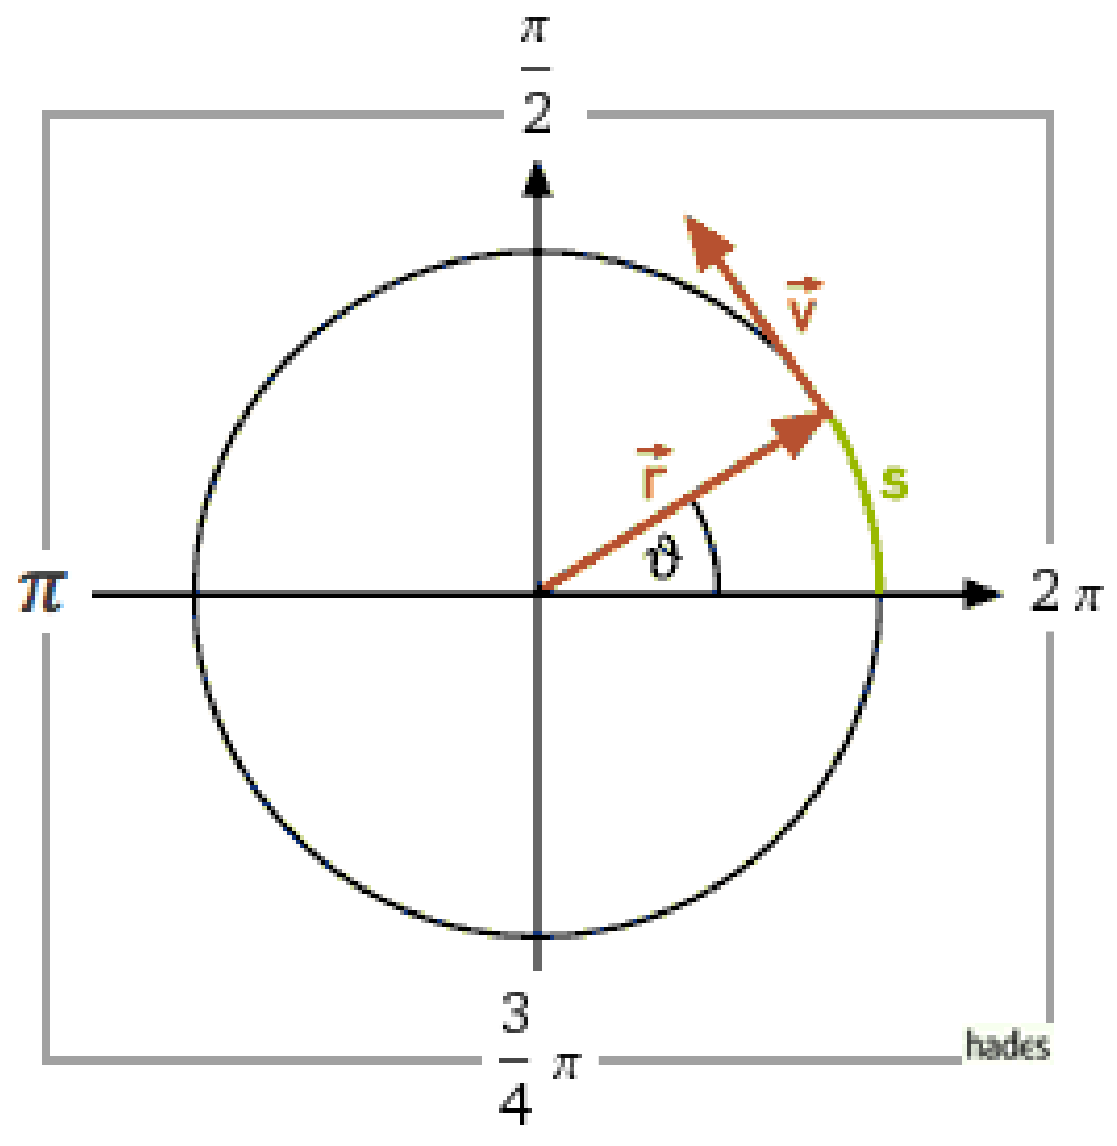
\includegraphics[width=0.2\linewidth]{images/rotation}

\paragraph{Konstante Geschwindigkeit (gleichförmig)}

\begin{tabbing}
	\begin{tabu} to \linewidth {l X l X}
		\toprule
		Winkelgeschwindigkeit & $\omega = \frac{\varphi}{t} = 2 \pi f$ &
		Rotationswinkel & $\varphi = \omega \cdot t$ \\
		Zeit & $t = \frac{\varphi}{\omega}$ &
		Drehzahl & $n = \frac{z}{t} = \frac{1}{T} = \frac{\omega}{2 \pi}$  \\
		Periodendauer & $T = \frac{1}{n} = \frac{2\pi r}{v} = \frac{2\pi}{\omega}$ &
		Anz. Umdrehungen & $N = \frac{\varphi}{2 \pi}$ \\
		\bottomrule
	\end{tabu}
\end{tabbing}

\paragraph{Konstante Beschleunigung (gleichmässig)}

\begin{tabbing}
	\begin{tabu} to \linewidth {l X X}
		\toprule
		& Ohne Anfangsgeschwindigkeit & Mit Anfangsgeschwindigkeit \\
		\midrule
		Winkelbeschleunigung & 
		$\alpha = \frac{\omega}{t} = \frac{2 \varphi}{t^2} = \frac{\omega^2}{2 \varphi}$ &
		$\alpha = \frac{\omega^2 - \omega_0^2}{2 \varphi}$ \\
		Winkelgeschwindigkeit & 
		$\omega = \alpha t = \sqrt{2 \alpha \varphi}$ &
		$\omega = \alpha t + \omega_0 = \sqrt{2\alpha \varphi + \omega_0^2} $ \\
		$\varnothing$ Winkelgeschwindigkeit & 
		$\omega_m = \frac{\alpha t}{2} = \frac{\varphi}{t}$ & \\
		Rotationswinkel & 
		$\varphi = \frac{\omega t}{2} = \frac{\omega^2}{2 \alpha} = \frac{\alpha t^2}{2} = \frac{s}{r} = 2\pi N$ &
		$\varphi = \frac{(\omega_0 + \omega_1)t}{2} = \frac{\omega^2 - \omega_0^2}{2 \alpha} = \frac{\alpha t^2}{2} + \omega_0 t + \varphi_0$ \\
	\end{tabu}
\end{tabbing}

\paragraph{Umrechnung Translation und Rotation}

\begin{tabbing}
	\begin{tabu} to \linewidth {l X l X l X}
		\toprule
		Geschwindigkeit & $v = r \cdot \omega$ &
		Beschleunigung & $a = r \cdot \alpha$ &
		Strecke & $s = r \cdot \varphi$ \\
		Winkelgeschwindigkeit & $\omega = \frac{v}{r}$ &
		Winkelbeschleunigung & $\alpha = \frac{a}{r}$ &
		Rotationswinkel & $\varphi = \frac{s}{r}$ \\
		\bottomrule
	\end{tabu}
\end{tabbing}

\begin{tabbing}
	\begin{tabu} to \linewidth {l X l}
		Variable & Bedeutung & SI-Einheit \\
		\midrule
		$\varphi$ & Rotationswinkels  & rad (Bogenmass) \\ 
		$\omega$ & Winkelgeschwindigkeit & $\frac{rad}{s}$ \\
		$\alpha$ & Winkelbeschleunigung & $\frac{rad}{s^2}$ \\
		$n = f$ & Drehzahl rsp. Umdrehungsfrequenz & $\frac{1}{s} = Hz$ \\
		$N$ & Anzahl ausgeführte Umdrehungen & \\
		$T$ & Periodendauer, Umlaufdauer & $s$ \\
		$t$ & Zeit die für die Drehung um den Winkel $\varphi$ benötigt wird & $s$ \\
		$s$ & Weg beim Umfang & $m$ \\
		$r$ & Radius & $m$ \\
		$z$ & Anzahl der Umdrehungen während der Zeit t & \\
		\bottomrule
	\end{tabu}
\end{tabbing}

\paragraph{Translation vs. Rotation}
\begin{tabbing}
	\begin{tabu} to \linewidth {l|l|l||l|l|l}
		\toprule
		& Translation & &  & Rotation &  \\ 
		\midrule
        S & Grösse & Beziehung & S & Grösse & Beziehung \\
        \midrule
        $s$ & Weg [$m$] & - & $\phi$ & Winkel [$rad$] & - \\ \hline
        $v$ & Geschwindigkeit [$\frac{m}{s}$] & $v=\frac{ds}{dt}$ & $\omega$ & Winkelgeschwindigkeit [$\frac{rad}{s}$] & $\omega = \frac{d\phi}{dt}$ \\ \hline
        $a$ & Beschleunigung [$\frac{m}{s^2}$] & $a=\frac{dv}{dt}$ & $\alpha$ & Winkelbeschleunigung [$\frac{rad}{s^2}$] & $\alpha = \frac{d\omega}{dt}$ \\ \hline
        $m$ & Masse [$kg$] & - & $J$ & Trägheitsmoment [$kg*m^2$] & - \\ \hline
        $\rho$ & Impuls [$N*s$] & $\rho = m * v$ & $L$ & Drehimpuls [$N * s$] & $L = J * \omega$ \\ \hline
        $F$ & Kraft [$N = \frac{kg*m}{s^2}$] & $F = \frac{dp}{dt}=m*a$ & $M$ & Drehmoment [$Nm$] & $M = \frac{dL}{dt} = J * \alpha$ \\ \hline
        $W$ & Arbeit [$J = N * m$] & $W = F * s$ & $W$ & Arbeit [$J = N * m$] & $W = M * \phi$ \\ \hline
        $P$ & Leistung [$W$] & $P = F*v = \frac{E}{t}$ & $P$ & Leistung [$W$] & $P = M * \omega$ \\ \hline
        $E$ & Translationsenergie [$J$] & $E_{trans} = \frac{m*v^2}{2}$ & $E$ & Rotationsenergie [$J$] & $E_{rot} = \frac{J*\omega^2}{2}$ \\ \hline
		\bottomrule
	 \end{tabu}
\end{tabbing}